\section{Approach}
\subsection{Simulated Network}

\subsection{Controller}

\subsubsection{Actuator}

\subsubsection{Sensor}

\subsubsection{Internet Cloud}

\subsubsection{Factory Access Point}

\subsubsection{Factory Bridge}

\subsection{MATLAB Simulation}
  We chose to use MATLAB simulation for the physical system and it's controls, 
  as there are many chemical process models currently implemented in MATLAB.
  This allows for the ease of swapping out current MATLAB models for new ones.

\subsubsection{Tennessee Eastman}
  In order to keep the complexity down, we decided to model the chemical process
  in the plant as a simplified Tenneessee Eastman problem\citation{Ricker}. 
  Due to this approach, we looked to previous work in the field, and found many
  models already modeled in a hybrid of FORTRAN and MATLAB.  However, this 
  introduced more complexity, due to using three different programming languages
  to implement what should be simpler.  Therefore, we would build a custom
  MATLAB function that contained the same functionality.

\subsection{C++ to MATLAB Bridge}
  

\begin{figure*}
        \centering
		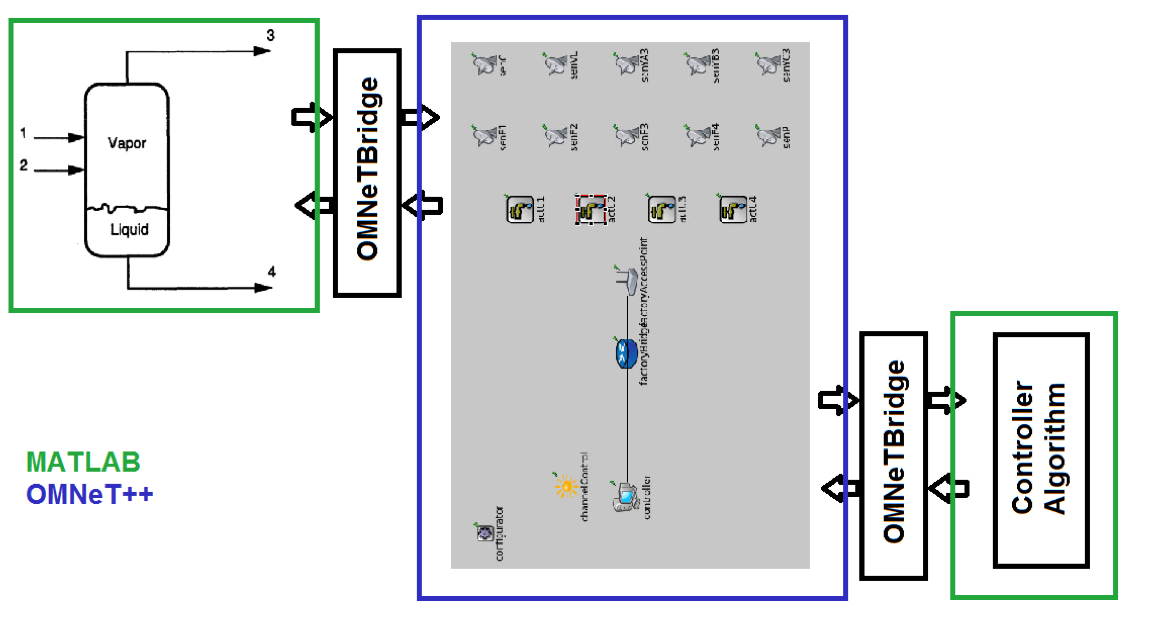
\includegraphics[width=0.8\textwidth]{figs/system.png}
        \caption{System Diagram.}
        \label{fig:system}        
\end{figure*}
